\documentclass[25pt, a0paper, portrait, margin=0mm, innermargin=15mm,blockverticalspace=15mm, colspace=15mm, subcolspace=8mm]{tikzposter}

\usepackage{fontspec}
\usepackage{multirow}

\defaultfontfeatures{PunctuationSpace=3,Scale=MatchLowercase,Mapping=tex-text}

\setromanfont{Liberation Serif}
\setmonofont{DejaVu Sans Mono}

\settitle{ \centering \vbox{
%\@titlegraphic \\[\TP@titlegraphictotitledistance] \centering
\color{titlefgcolor} {\bfseries \Huge \sc \@title \par}
\vspace*{1em}
{\huge \@author \par} \vspace*{1em} {\LARGE \@institute}
}}

\makeatletter
\def\title#1{\gdef\@title{\scalebox{\TP@titletextscale}{%
\begin{minipage}[t]{0.7\linewidth}
\centering
#1
\par
\vspace{0.5em}
\end{minipage}%
}}}
\makeatother

\title{Unsupervised training of maximum-entropy models 
 for lexical selection in rule-based machine translation}
 \institute{$^\star$UiT Norgga árktalaš universitehta, $^\dagger$Universitat d'Alacant} % See Section 4.1
\author{Francis M. Tyers,$^\star$ Felipe Sánchez-Martínez,$^\dagger$ Mikel L. Forcada$^\dagger$} 
%\titlegraphic{
%\includegraphics[width=0.04\textwidth]{LogoSamisk.png} \hspace{20pt}
%
\includegraphics[width=0.15\textwidth]{logodlsioficialcolor.eps} 
%}
\usetheme{Basic} % See Section 5
\begin{document}


\maketitle % See Section 4.1
\begin{columns} % See Section 4.4
\column{0.45} % See Section 4.4
\block{BlocktitleB}{Blocktext}
\column{0.55}
\block{BlocktitleC}{
\begin{center}
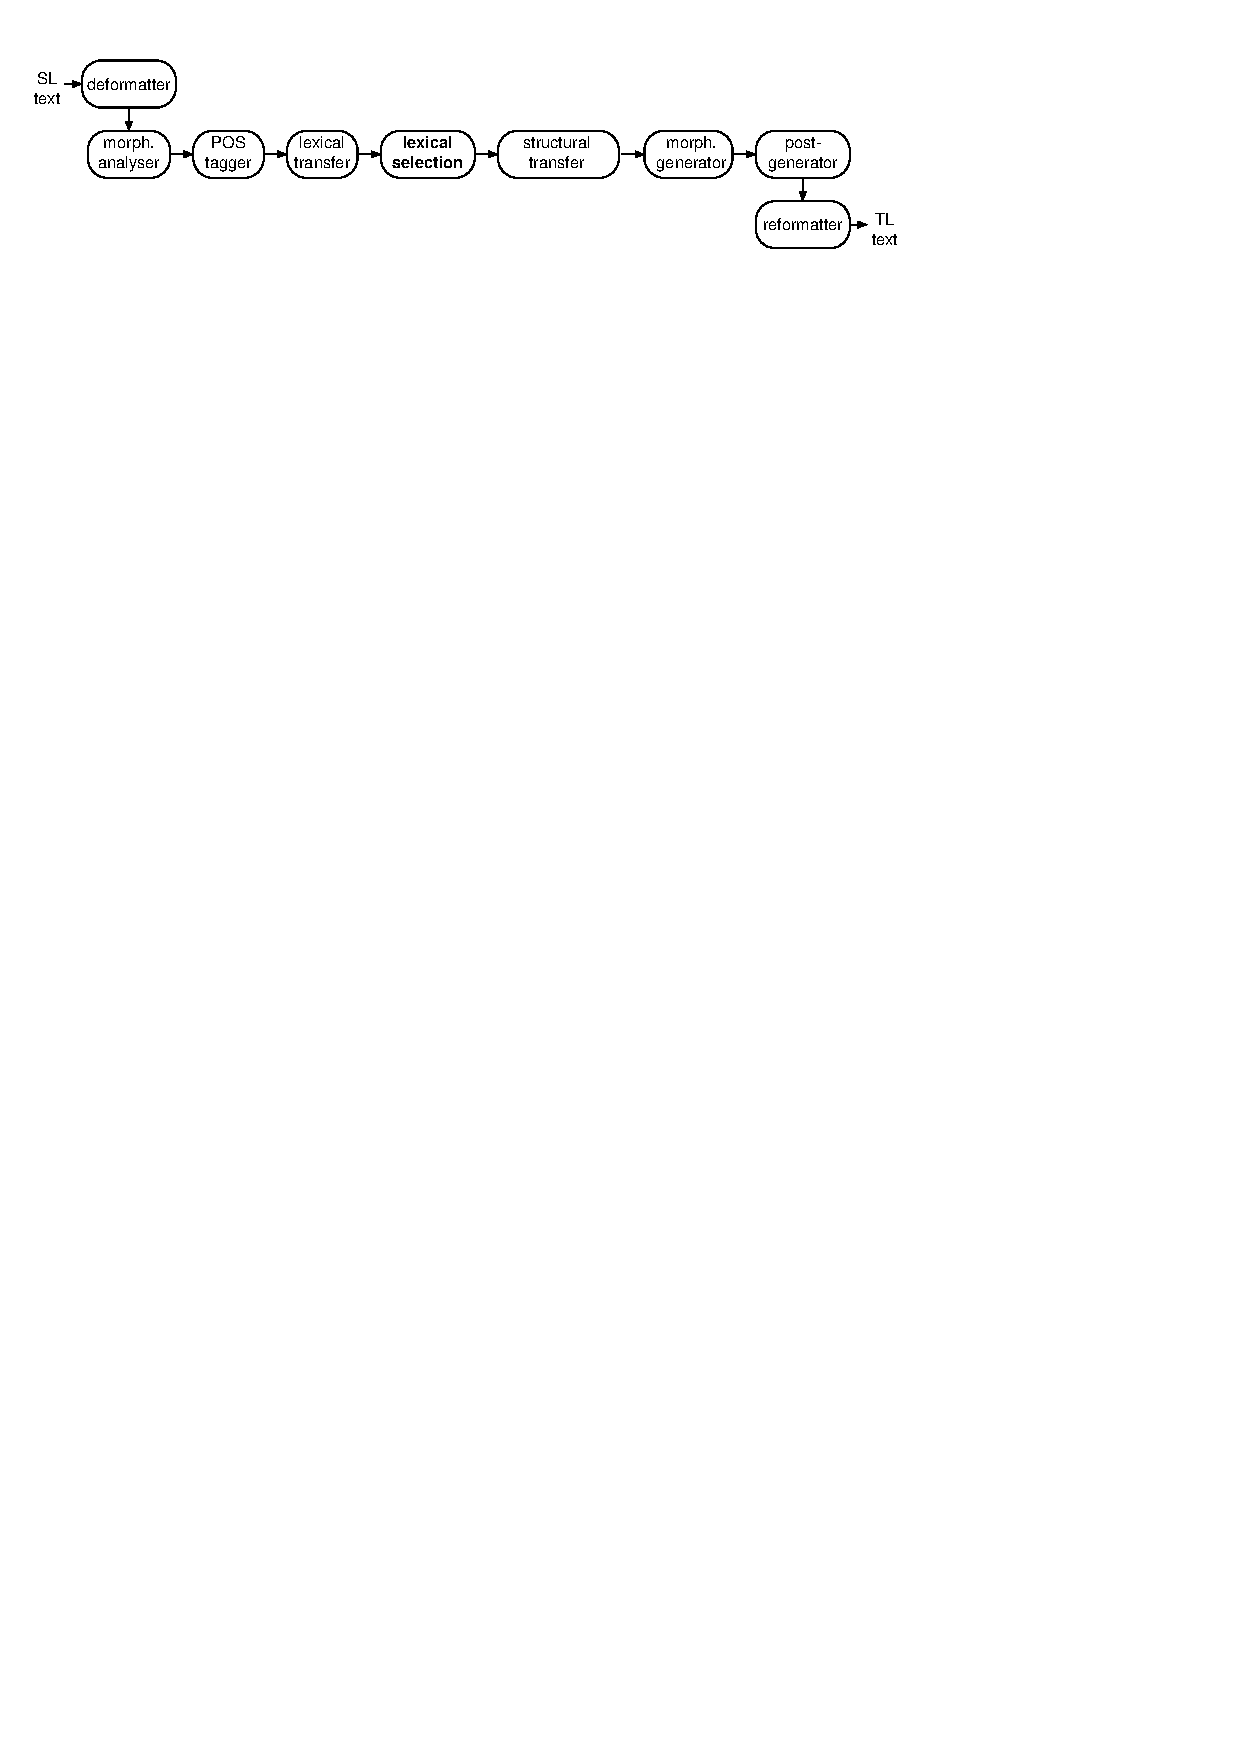
\includegraphics[width=0.5\textwidth]{architecture-lexsel.pdf}
\end{center}
}
%\note{Notetext} % See Section 4.3
\end{columns}
\begin{columns} % See Section 4.4
\column{0.45} % See Section 4.4
\block{BlocktitleB}{\begin{displaymath}
  \label{eq:steps}
  S \to \mbox{\framebox{\parbox{4.0cm}{\textit{pre-lexsel}}}} \to (\{g_i\}_{i=1}^{i=|G|},S) \to \mbox{\framebox{\parbox{3.5cm}{\textit{\textbf{lexsel}}}}} \to (g^\star,S) \to \mbox{\framebox{\parbox{4.0cm}{\textit{post- lexsel}}}} \to \tau(g^\star,S)
\end{displaymath}
}

\column{0.55}
\block{BlocktitleA}{ % See Section 4.2
\useinnerblockstyle{Table}
\begin{center}
\begin{tabular}{|c|l|r|}
     \hline
        & \textbf{Sentence} & $p(g_i|S)$ \\
     \hline % Los pescados grandes peque\~{n}o come
      \(S_1\) & \emph{Arrain handiak txikia jaten du}  &  \\
                         $\tau(g_{11},S_1)$ & El pez grande se come el peque\~{n}o &  0.830 \\
                         $\tau(g_{12},S_1)$ & El pescado grande se come el peque\~{n}o & 0.134 \\
                         $\tau(g_{13},S_1)$ & El pescado capaz se come el peque\~{n}o & 0.034\\
                         $\tau(g_{14},S_1)$ & El pez capaz se come el peque\~{n}o  & 0.001\\
     \hline % El padre el pescado nos ha preparado para cenar
      \(S_2\) & \emph{Aitak arraina prestatu digu afaltzeko} &  \\
                         $\tau(g_{21},S_2)$ & Padre nos ha preparado pescado para cenar & 0.846 \\
                         $\tau(g_{22},S_2)$ & Pap\'{a} nos ha preparado pescado para cenar & 0.134 \\
                         $\tau(g_{23},S_2)$ & Padre nos ha preparado pez para cenar & 0.015 \\
                         $\tau(g_{24},S_2)$ & Pap\'{a} nos ha preparado pez para cenar & 0.005 \\
     \hline % Aqu\'{\i} el pescado muy es dulce
     $S_3$  & \emph{Hemen arraina oso goxoa da}  & \\
                         $\tau(g_{31},S_3)$ & Aqu\'{\i} el pescado es muy rico & 0.912 \\
                         $\tau(g_{32},S_3)$ & Aqu\'{\i} el pescado es muy suave & 0.067 \\
                         $\tau(g_{33},S_3)$ & Aqu\'{\i} el pez es muy rico & 0.011 \\
                         $\tau(g_{34},S_3)$ & Aqu\'{\i} el pez es muy suave & 0.008 \\
                         $\tau(g_{35},S_3)$ & Aqu\'{\i} el pez es muy dulce & 0.001 \\
                         $\tau(g_{36},S_3)$ & Aqu\'{\i} el pescado es muy dulce & 0.001 \\
     \hline % Un pescado grande del mar es
     \(S_4\) & \emph{Itsasoko arrain handi bat da} & \\
                         $\tau(g_{41},S_4)$ & Es un pez grande del mar & 0.595 \\
                         $\tau(g_{42},S_4)$ & Es un pescado grande del mar & 0.403 \\
                         $\tau(g_{43},S_4)$ & Es un pez capaz del mar & 0.001 \\
                         $\tau(g_{44},S_4)$ & Es un pescado capaz del mar & 0.001 \\
     \hline % El pescado grande por esos serv\'{\i}an para alimentar
     $S_5$ &  \emph{Arrain handiak horiez baliatzen ziren elikatzeko} &  \\
                         $\tau(g_{51},S_5)$ & Los peces grandes se nutr\'{\i}an de esos & 0.862 \\
                         $\tau(g_{52},S_5)$ & Los pescados grandes se nutr\'{\i}an de esos & 0.121 \\
                         $\tau(g_{53},S_5)$ & Los peces grandes se alimentaban de esos & 0.012 \\
                         $\tau(g_{54},S_5)$ & Los peces capaces se alimentaban de esos & 0.001 \\
                         $\tau(g_{55},S_5)$ & Los pescados grandes se alimentaban de esos & 0.001 \\
                         $\tau(g_{56},S_5)$ & Los pescados capaces se alimentaban de esos & 0.001 \\
                         $\tau(g_{57},S_6)$ & Los peces capaces se nutr\'{\i}an de esos & 0.001 \\
                         $\tau(g_{58},S_7)$ & Los pescados capaces se nutr\'{\i}an de esos & 0.001 \\
     \hline
   
   \end{tabular}
\end{center}
}
\end{columns}
\block{Results}{ % See Section 4.2
 \begin{center}

  \begin{tabular}{|l|l|r|r|r||r|}
    \hline
    \multirow{2}{*}{{\bf Pair}}  & \multirow{2}{*}{{\bf Metric}} & \multicolumn{4}{|c|}{{\bf System}} \\ \cline{3-6}
                                 &              & {\tt Ling} & {\tt TLM} & \texttt{MaxEnt} & \texttt{Oracle} \\
    \hline % tlm-alig: [44.5, 50.2]
    \multirow{2}{*}{{\bf br-fr}} & {\sc ler} (\%)     & [54.8, 60.7] & [44.2, 50.5]  & {\bf [40.8, 46.9]} & [0.0, 0.0]      \\ 
                                 & {\sc bleu} (\%)    & [14.5, 16.4] & [15.4, 17.3]  & [14.8, 16.6] & [16.7, 18.6]     \\ 
    \hline % tlm-alig: 
    \multirow{2}{*}{{\bf mk-en}} & {\sc ler} (\%)     & [28.8, 32.6] & [26.8, 30.5]  & [25.2, 28.8] & [0.0, 0.0]    \\ 
                                 & {\sc bleu} (\%)    & [28.6, 31.0] & [30.7, 32.3]  & [29.1, 31.5] & [30.9, 33.3]    \\ 
    \hline % tlm-alig: 
    \multirow{2}{*}{{\bf eu-es}} & {\sc ler} (\%)      & [43.6, 48.8] & [38.8, 44.2]  & [40.9, 46.2] & [0.0, 0.0]     \\ 
                                 & {\sc bleu} (\%)     & [10.1, 12.0] & [10.6, 12.6]  & [10.3, 12.2] & [11.5, 13.5]     \\ 
    \hline % tlm-alig: [10.3, 13.9]
    \multirow{2}{*}{{\bf en-es}} & {\sc ler} (\%)      & [20.5, 24.9] & [15.1, 18.9]  & {\bf [10.4, 13.8]} & [0.0, 0.0]     \\ 
                                 & {\sc bleu} (\%)     & [21.5, 23.4] & [21.9, 23.8]  & {\bf [22.2, 24.1]} & [22.8, 24.7]     \\ 
    \hline
  \end{tabular}

 \end{center}

}
\end{document}
